\chapter{Snapshot}
\label{chap:snapshot}
    One of the major features of the Kabi File System is writable copy-on-write snapshot. Snapshot nodes are designed to be one of the basic component of the Kabi File System. The “current” status of the file system is also treated as a writable snapshot. This lightweight snapshot system focuses on reducing the storage space occupied by a snapshot.

    In a snapshot system, most snapshots do not keep a copy of the entire file system but instead they will log the changes since the last snapshot. In this way the snapshot system can rebuild the content of the a snapshot based on the previous snapshot and the log of changes, as shown in \fref{fig:snapshot_patch} The only exception is a unique snapshot called root snapshot which references the entire file system. All other snapshots contain a reference to another snapshot and list of patch nodes. Each patch node in the list reflects a change or a series of changes on the one file node or one directory node since the last snapshot.

    (ADD LONG TERM IMPACT)

\begin{figure}[hbtp]
\centering
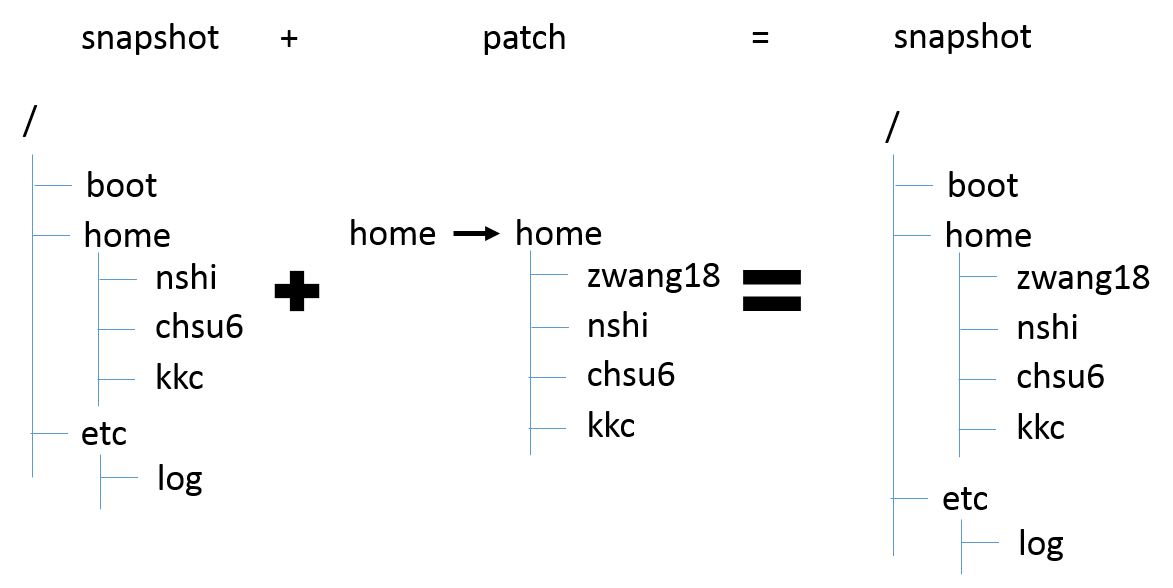
\includegraphics[width=0.8\textwidth]{Chapter-4/figs/fig23.png}
\caption{Snapshots and Patches}
\label{fig:snapshot_patch}
\end{figure}

\section{The Snapshot Tree}

	The snapshot system in Kabi File System uses a lightweight approach based on patches. Some other snapshot file system like SnapFS and ext3cow uses a reserved field in inode to reference the previous version inode shown in \fref{fig:snapfs_approach}. Compared to that approach, the patch based mechanism is not only more efficient in snapshot read access but also supports tree structured snapshots and writable snapshots.

\begin{figure}[hbtp]
\centering
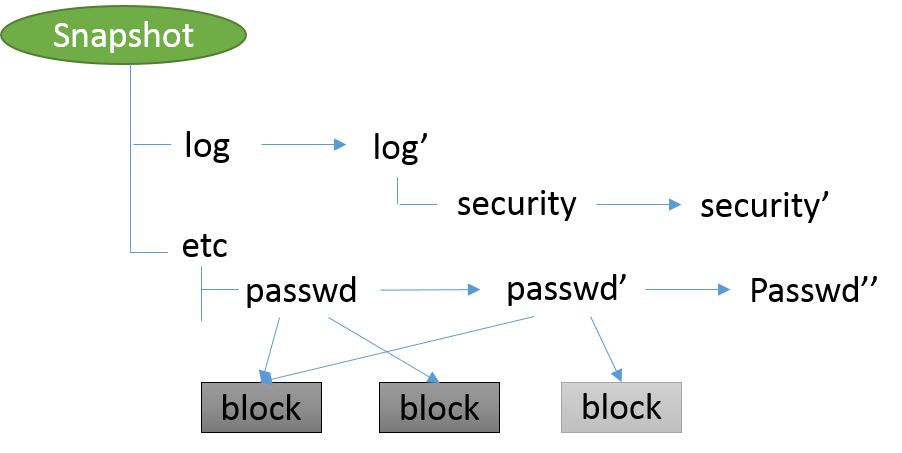
\includegraphics[width=0.7\textwidth]{Chapter-4/figs/fig24.png}
\caption{Snapshots in SnapFS}
\label{fig:snapfs_approach}
\end{figure}

    Snapshots in the Kabi File System are represented by snapshot node and forms an up-tree. The following \fref{fig:snap_tree_example} shows an example of the snapshot tree.

\begin{figure}[hbtp]
\centering
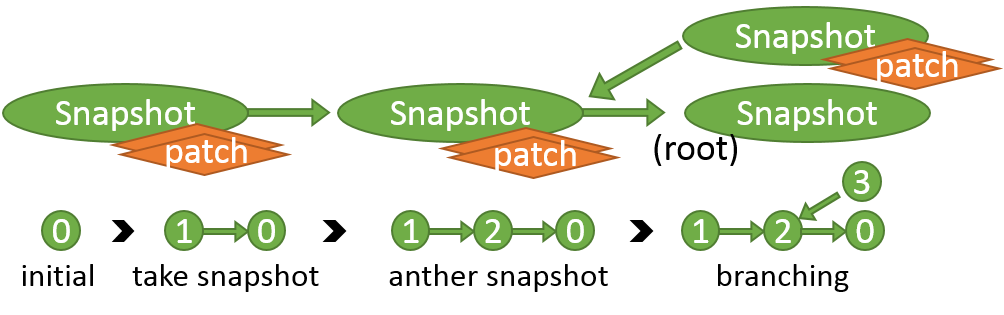
\includegraphics[width=0.8\textwidth]{Chapter-4/figs/fig13.png}
\caption{An example of snapshot tree}
\label{fig:snap_tree_example}
\end{figure}

    At initial status, the file system contains a default writeable snapshot node (node \#0 in \fref{fig:snap_tree_example}) representing the current status of the file system. This unique snapshot called the root snapshot is the only snapshot node that does not reference other snapshot. For initial status, writes to the file system go directly into the root snapshot.
    
    After a snapshot is taken, a new snapshot node (node \#1) is created referring to the root snapshot node. Subsequent write operations will not only write data into the root snapshot but also submit patches to all snapshot connected to root snapshot, so as to reflect the difference between snapshot node \#1 and its referencing node \#0.

    Branching a snapshot is equivalent to creating a new snapshot node referring the snapshot being forked. As shown in \fref{fig:snap_tree_example}, node \#3 is created and connected to snapshot node \#2 in order to branch the file system based on snapshot \#2.

    In the snapshot tree, the main branch is the branch that contains root snapshot node. All other branches are side branches. In a branch, the latest snapshot node represents the “current status” of the file system of this branch. Other snapshot nodes forms the historical status of their corresponding branch. \fref{fig:branches} shows the idea of branch

\begin{figure}[hbtp]
\centering
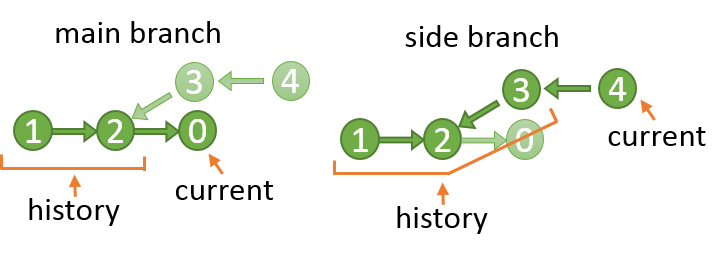
\includegraphics[width=0.65\textwidth]{Chapter-4/figs/fig22.png}
\caption{Branches}
\label{fig:branches}
\end{figure}

\section{Nodes}

    As mentioned in previous section, there are two types of snapshot node in this file system, namely the root snapshot node and the non-root snapshot node.

    The root snapshot is unique in the file system. It is the root of the up-tree (CITE HERE OR EXPLAIN) and does not reference any other snapshot. Instead it stores the content of the entire file system by referencing the directory node of the root directory. In this way, read access to root snapshot node is intuitive and faster than any other snapshot, so root snapshot is recommended to be used to represent the most frequently accessed snapshot or the current status of the file system.

    On the other hand, a non-root snapshot does not have their own root directory but keeps a reference to another snapshot node and a list of patch nodes which represent the difference between this non-root snapshot and the referenced snapshot. Reading a non-root snapshot will first read the corresponding content in referenced snapshot and then lookup the patch list to find out if the content is marked as changed in this snapshot. To write the non-root snapshot upload the changed nodes into the database and pack their id into a patch node and submit the patch. Be aware that not all non-root snapshots are writable, once the non-root snapshot is referenced by some other snapshot nodes, it becomes immutable.

    \fref{fig:root_and_nonroot} shows a root snapshot node (right) and a non-root snapshot (left).
    
\begin{figure}[hbtp]
\centering
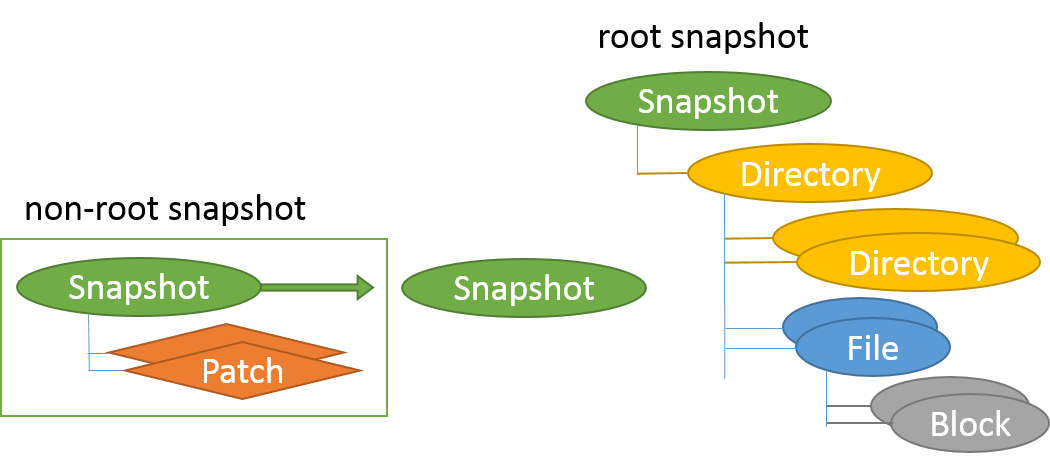
\includegraphics[width=0.75\textwidth]{Chapter-4/figs/fig12.png}
\caption{Root Snapshot and Non-root Snapshot}
\label{fig:root_and_nonroot}
\end{figure}

    A patch node reflects a series of changes to one file or one directory node. It references a pair of file nodes or directory nodes. The two nodes referred are the target node (original version) and its replacement (changed version).

    \fref{fig:patches} demonstrates the way patch works. Snapshot 1 and 2 demonstrates how a directory is changed between snapshots. The directory that was represented by node $d_2$ in snapshot 2 is now replaced by directory node $d_1$ in snapshot 1. In snapshot 2, the directory has a new subdirectory but the file under that directory remains unchanged. Hence the target node (node $d_2$) and replacement node (node $d_1$) have a reference to a same file node but the target node $d_2$ has one more reference to a directory node. In the example of snapshot ($a$) and snapshot ($b$), a file is changed in both snapshot, its original version is $f_1$, the intermedia version in snapshot ($b$) is $f_2$ and final version is $f_3$ in snapshot ($a$). In snapshot $\alpha$ and snapshot $\beta$, file $f_3$ is replaced by $f_2$ in snapshot ($\beta$) and replaced by $f_1$ in snapshot ($\alpha$).  

\begin{figure}[hbtp]
\centering
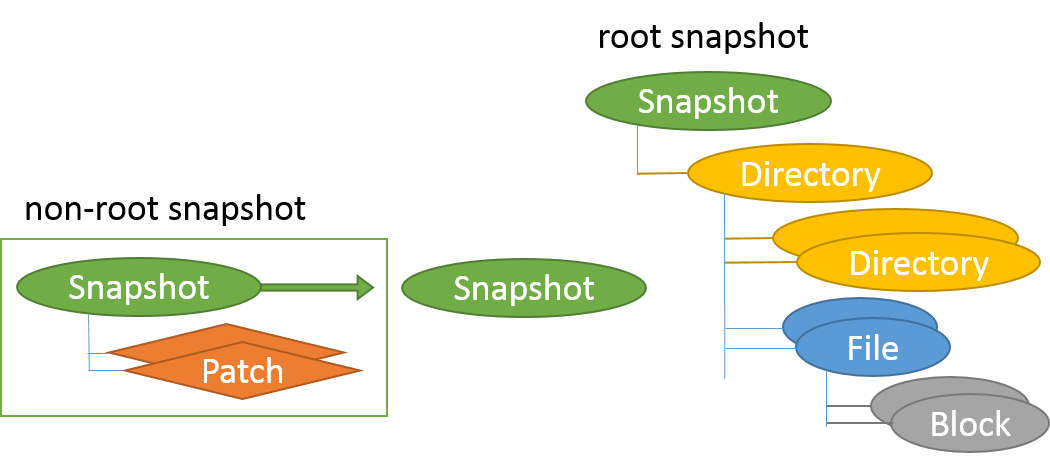
\includegraphics[width=0.75\textwidth]{Chapter-4/figs/fig12.png}
\caption{The Principle of Patches}
\label{fig:patches}
\end{figure}

\section{Operations}
\subsection{Read operations}

    When reading a file or a directory in non-root snapshot, the file system must to do a lot of lookup in patch lists to ensure we are reading the correct version of the node. For instance, in \fref{fig:read_patches} , to read the file “/a/d.txt” in snapshot \#1 shown in figure below, the file system will first read in “/” directory in root snapshot which is node \#3) . Then transverse all involved snapshots (\#1 and \#2) to see if there’s a patch whose target node is node \#3. Since no such patch is found, this means node \#3 is the “/” directory node of all snapshot node (\#1, \#2 and \#3). Then the file system will look for “a” directory under node \#3 and corresponding patches. In this example, there is a directory (node \#9) with display name “a” under node \#3 but there is also a patch to node \#9 in snapshot \#2. That means node \#5 is the “/a” directory node of snapshot \#0 while node \#6 is the directory node for snapshot \#1 and snapshot \#2. Follow the same procedure, we will find node \#8 is the “/a/d.txt” node in snapshot \#2 but for snapshot \#1 “/a/d.txt” represented by node \#6.

\begin{figure}[hbtp]
\centering
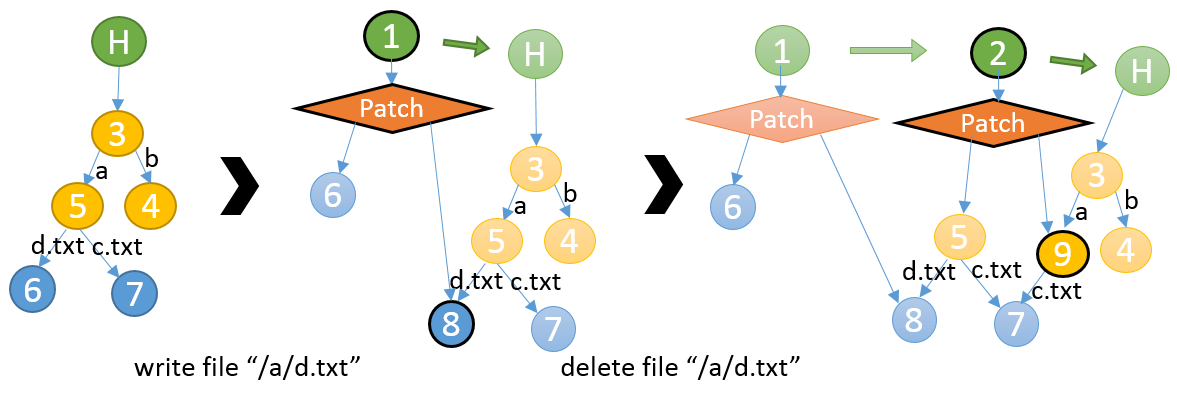
\includegraphics[width=0.5\textwidth]{Chapter-4/figs/fig18.png}
\caption{Read a snapshot}
\label{fig:read_patches}
\end{figure}

    As one can see, read operations deeply rely on the patch lookup operation. To avoid query and traverse all involved snapshot nodes and patch nodes on every a read operation, a runtime patch list is built and stored as hashtable in memory when a non-root snapshot node is mounted. The runtime patch list combines all patches that may be used for a node lookup. In the example shown in \fref{fig:combine_patch_list}, when mounting snapshot \#3, a runtime patch list that contains all effective patches in snapshot \#3 and \#2 is created.

\begin{figure}[hbtp]
\centering
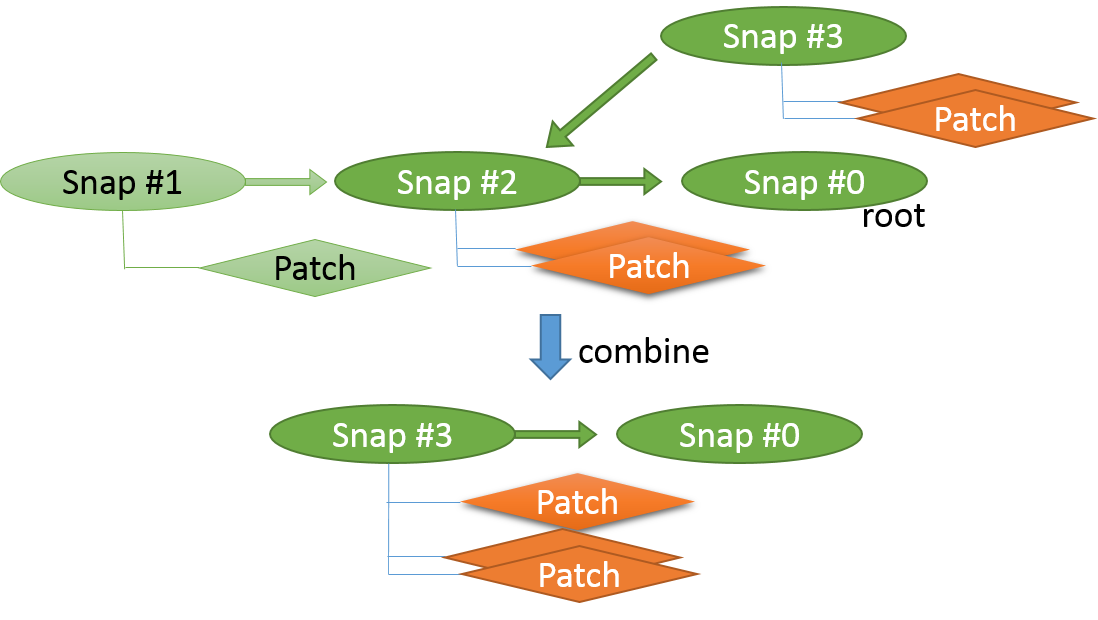
\includegraphics[width=0.8\textwidth]{Chapter-4/figs/fig15.png}
\caption{Combine Patch Lists}
\label{fig:combine_patch_list}
\end{figure}

    Not all patches in patch lists will be combined into the runtime patch list. Some patches are mergeable and some are duplicated. For instance, in \fref{fig:merge} snapshot (a) and (b) the replacement node of a patch is also the target node of another patch, these two patch node can be merged into one runtime patch. Another example is snapshot ($\alpha$) and ($\beta$), when two patch nodes have the same target node, they are duplicated and one of them can be discarded.

\begin{figure}[hbtp]
\centering
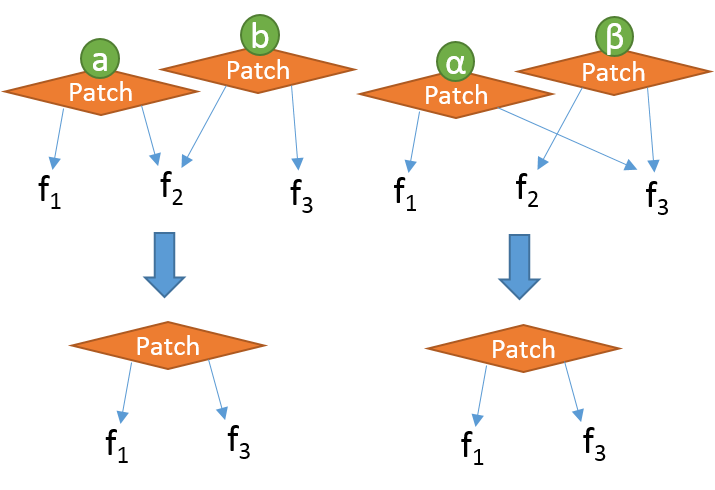
\includegraphics[width=0.7\textwidth]{Chapter-4/figs/fig19.png}
\caption{Merge Patches}
\label{fig:merge}
\end{figure}

\subsection{Write operations}

	\fref{fig:create_snapshots} below briefly demonstrates how patch node and snapshots work with write operations. This example has 3 snapshots. node \#0 is the root snapshot node representing the current status of the main branch. Snapshot node \#2 represents the initial status and node \#1 is the intermediate status of main branch. At initial status, the file system contains three directory “/”, “/a”, “/b” and two files “/a/c.txt”, “/a/d.txt”. In between the initial snapshot and the next snapshot, file “/a/d.txt” was overwritten so its representing node is changed by a patch. After snapshot 2 is taken, the file “/a/d.txt” was deleted. A new patch is attached to snapshot 2 to reflect this change.

\begin{figure}[hbtp]
\centering
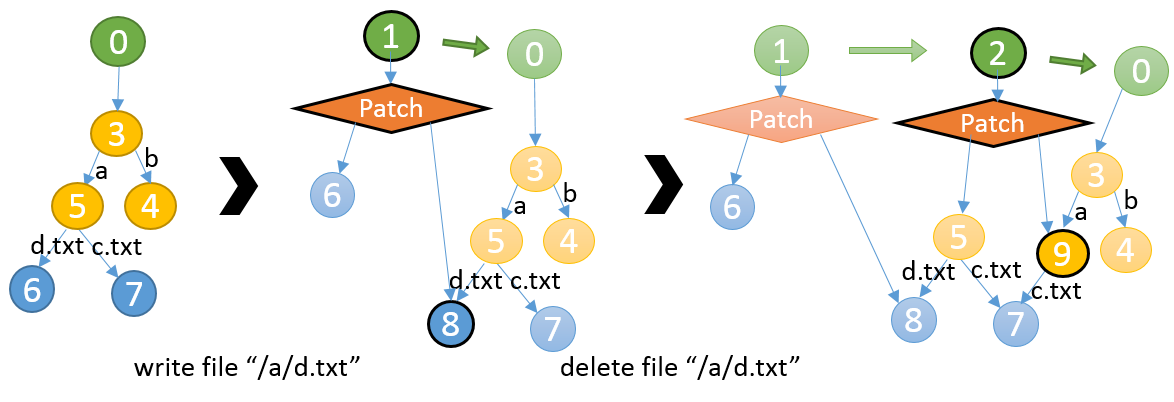
\includegraphics[width=0.95\textwidth]{Chapter-4/figs/fig26.png}
\caption{Example: Create Snapshots}
\label{fig:create_snapshots}
\end{figure}

    \fref{fig:take_snapshot_root} and \fref{fig:take_snapshot_nonroot} shows how to take a snapshot on main branch and side branch.

    In order to take a new snapshot on main branch, the file system will create a new snapshot node in between the root snapshot and its adjacent snapshot node. This newly created snapshots will have an empty patch list referencing the root snapshot. This new snapshot node will represent the status of this branch at the time it is created. While the current status of the main branch is still the root snapshot.

\begin{figure}[hbtp]
\centering
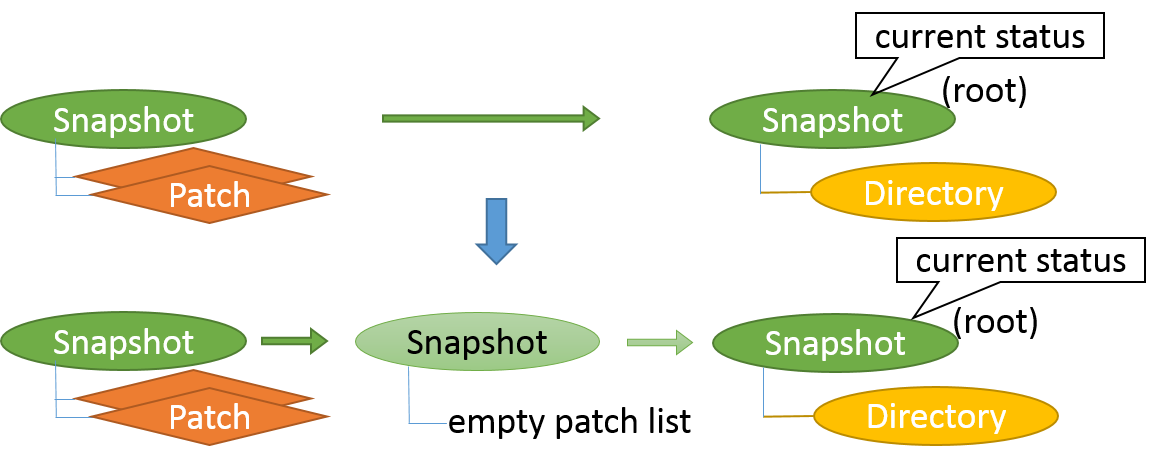
\includegraphics[width=0.8\textwidth]{Chapter-4/figs/fig20.png}
\caption{Take Snapshots on Main Branch}
\label{fig:take_snapshot_root}
\end{figure}
    
	To take a snapshot on a side branch, the file system will create a new snapshot node attached to the end of the side branch. The newly created snapshot node will reference the latest snapshot on this branch and have an empty patch list. After attached to the branch, this snapshot will become the current status of this branch.

\begin{figure}[hbtp]
\centering
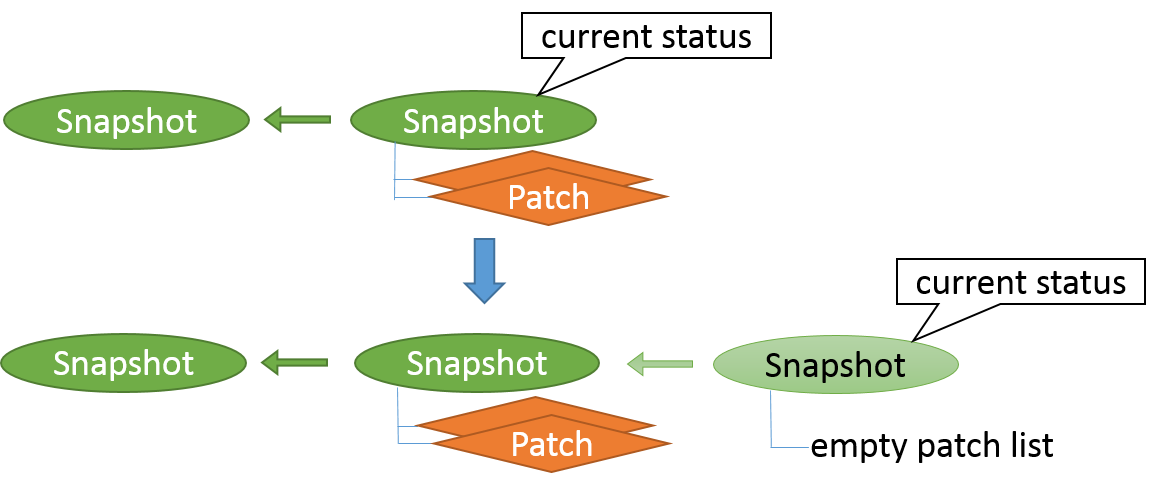
\includegraphics[width=0.8\textwidth]{Chapter-4/figs/fig21.png}
\caption{Take Snapshots on Side Branch}
\label{fig:take_snapshot_nonroot}
\end{figure}
    
    When writing a non-root leaf snapshot, the Kabi File System will submit new patches to that non-root snapshot to reflect the change. In the first example shown in \fref{fig:write_snapshot_node}, the file system is writing the root snapshot in main branch, replacing node X with its newer version Y. Node Y will replace node X directly in the root snapshot. In order to keep its previous version X in snapshot \#2, a “reverse” patch node will be submitted to revert node Y back to its original version X. In this way, the root snapshot have the new version Y while all other snapshots keep the old version X.  In the second example, the file system is trying to replace node X with its new version Y in snapshot \#3. This time it can simply submit a X->Y patch to snapshot \#3. In the third example, we demonstrate a walk around to writing an internal snapshot node by creating a branch based on that internal node and write to that branch.

\begin{figure}[hbtp]
\centering
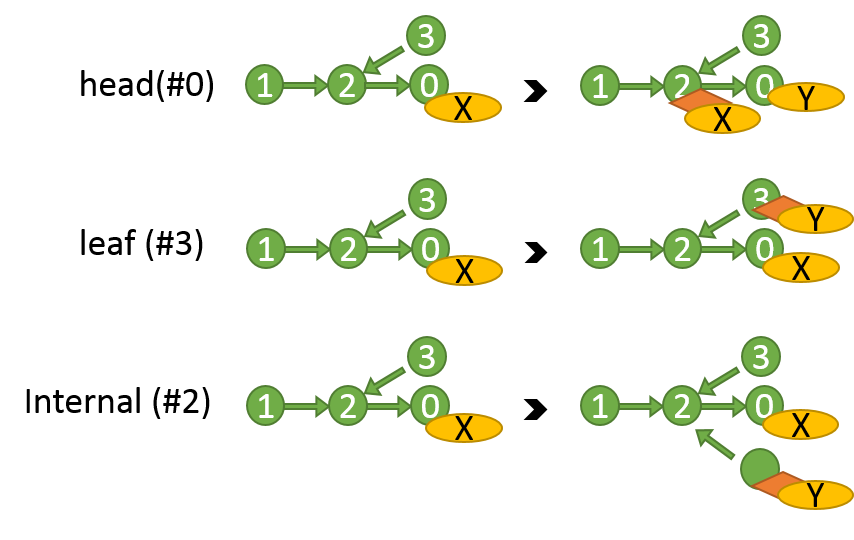
\includegraphics[width=0.7\textwidth]{Chapter-4/figs/fig17.png}
\caption{Write a Snapshot Node}
\label{fig:write_snapshot_node}
\end{figure}

    To create a branch based on the root snapshot, It is recommended to create a dummy snapshot first and then fork from that dummy node instead of branching the root snapshot directly. This is because write operation to root snapshot will submit patches to all connected snapshot nodes and we wish to limit the number of snapshots connected to the root snapshot. If we fork the root snapshot directly then there will be multiple snapshot node connected on to the root snapshot node. \fref{fig:dummy_node} demonstrates this issue:

\begin{figure}[hbtp]
\centering
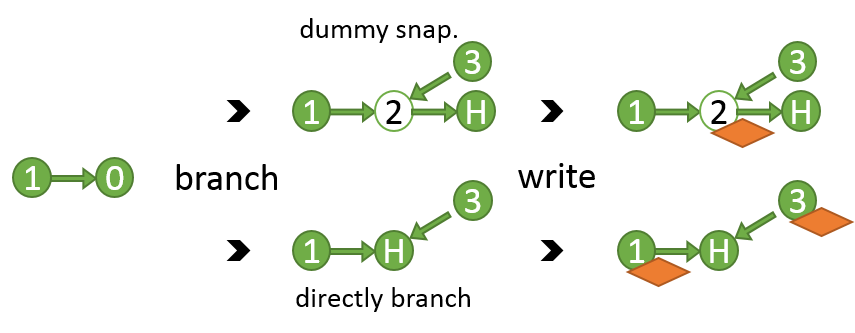
\includegraphics[width=0.8\textwidth]{Chapter-4/figs/fig16.png}
\caption{Branching Root Snapshot Node}
\label{fig:dummy_node}
\end{figure}

	Generally, within a shanshot, each node (file or directory) should have no more than one patch associate with it. For example, a patch replacing node 0 with node 1 and a patch replacing node 1 with  node 2 can be merged into one patch. This happens when a node is modified multiple times. For time and space efficiency, it is recommended to merge them into one patch.
	
\section{Enhancing Copy-on-Write and Deduplication}

	The copy-on-write strategy and file system deduplication improve space efficiency of the file system. File system deduplication finds and eliminates duplicated blocks and files while the classical copy-on-write strategy eliminates unnecessary copy of an unchanged block to snapshots.

\subsection{Motivation}

    A classical copy-on-write snapshot system applies copy-on-write at block level. As shown in \fref{fig:classic_cow}, Unchanged blocks will not be copied to the snapshot.

\begin{figure}[hbtp]
\centering
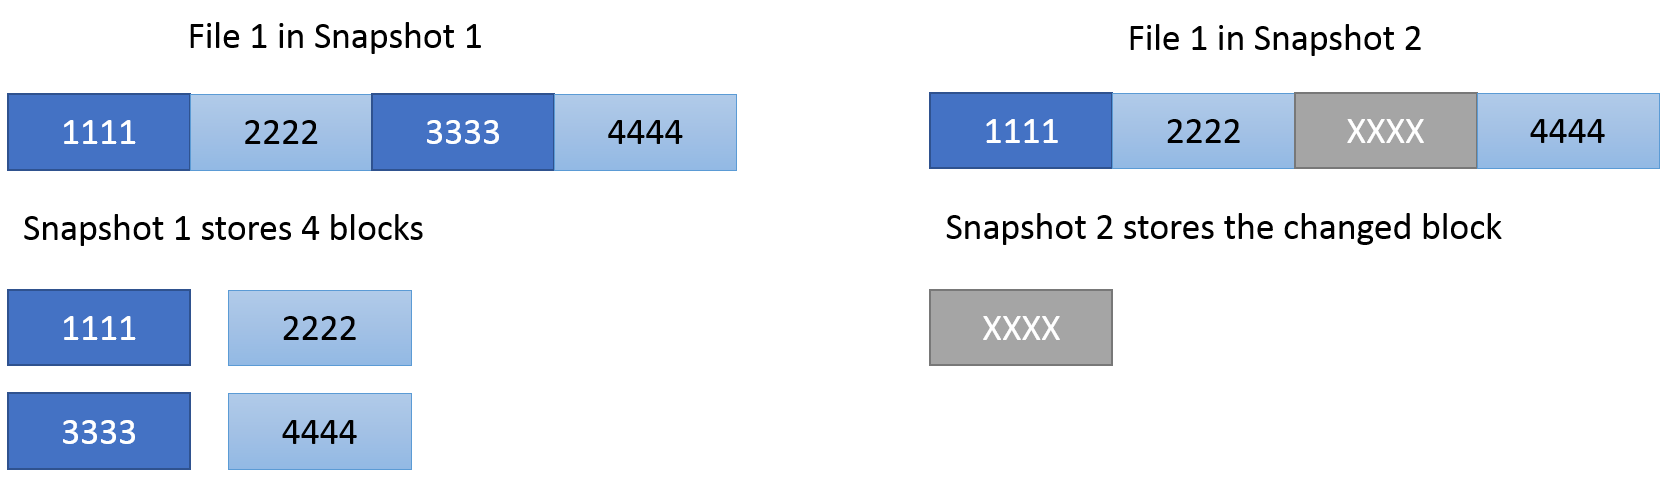
\includegraphics[width=0.8\textwidth]{Chapter-4/figs/fig4.png}
\caption{Classic Copy-on-Write}
\label{fig:classic_cow}
\end{figure}

    However, in reality it is not always an ideal solution. In many use cases like insertion or deletion, only a few bytes is affected instead of a whole block. In these scenarios, all successor blocks will be rewriten. The classical snapshot system will make a copy of all successor blocks despite the fact that only very few bytes is changed. The following \fref{fig:issue_classic_cow} addresses this issue. A byte is inserted into the file at offset 8. In classical copy-on-write snapshot system, 2 successor blocks are treated as changed blocks and will be copied. However, as we can see, the data in those blocks did not change but moved one byte forward. There could be a better solution.

\begin{figure}[hbtp]
\centering
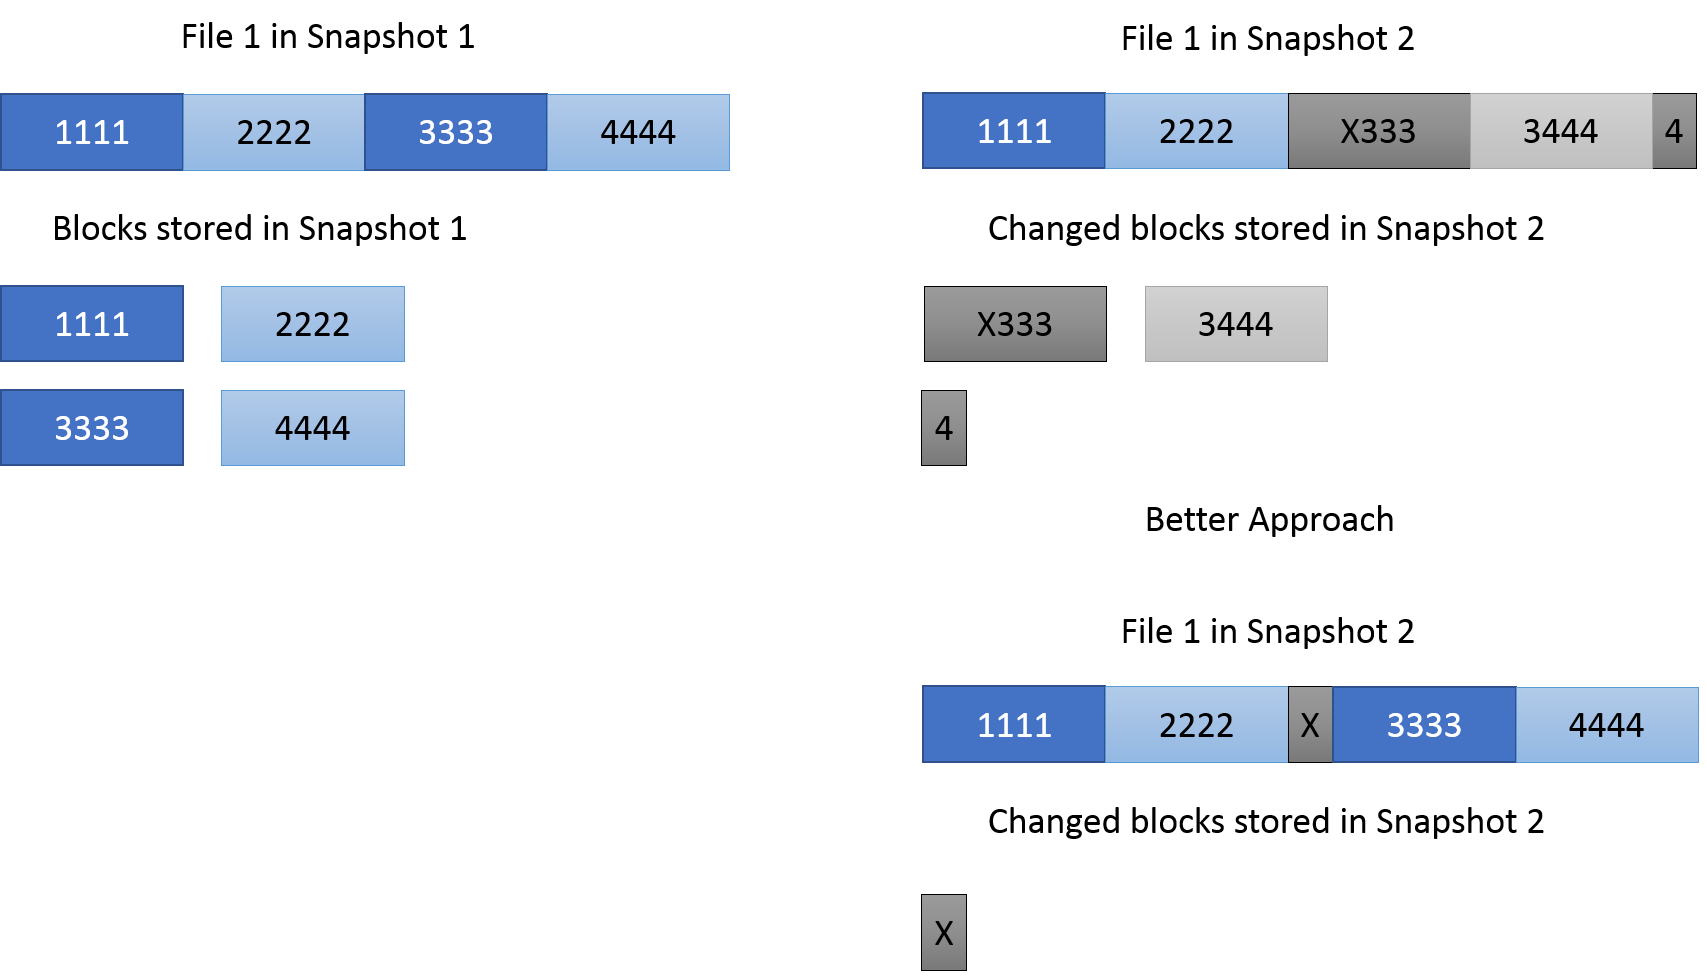
\includegraphics[width=0.8\textwidth]{Chapter-4/figs/fig5.png}
\caption{Issue in Classic Copy-on-Write}
\label{fig:issue_classic_cow}
\end{figure}
 
    To solve this problem, we have to let the file system be aware of the true intention of the end user. This is not straightforward because the POSIX standard uses only one file system call to handle all kinds of modification to a file. The only function of this file system call is to rewrite a part of a file.
    
    If the user program intent to insert a byte right in the middle of the file, the file system will receive a set of write calls to rewrite all later blocks to move original data 1 byte forward. The same behavior can also be observed when user program trying to rewrite the later half of the file. It is hard for the file system to distinguish these two scenario. Although sometimes we can use patterns to guess the intention of an operation, like an insertion usually results in a write() call after a truncate() call, we believe it’s better not to depend on those patterns or make any assumption on how the user program will behave. Therefore our major challenge is to identify the true intention of an write operation, is it an insertion or a complete rewrite?

\begin{figure}[hbtp]
\centering
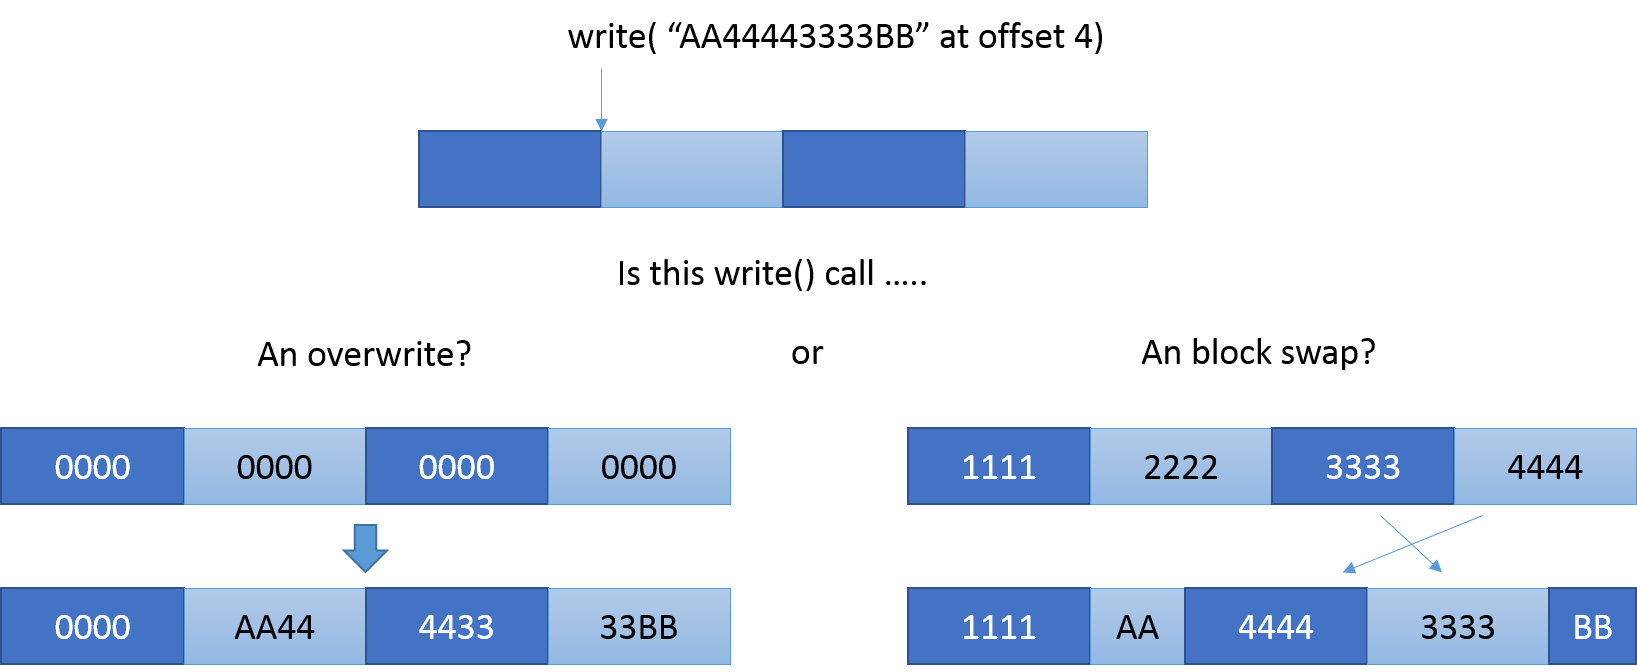
\includegraphics[width=0.8\textwidth]{Chapter-4/figs/fig6.png}
\caption{Identify the intention of write operations}
\label{fig:write_intention}
\end{figure}

\subsection{The rsync algorithm}

    As discussed in the previous section, we need to have a mechanism to compare the data to be written into the file and the original data to identify duplication. We use the rsync algorithm to accomplish this goal. It is originally designed for the efficient update of data over a high latency and low bandwidth link.

    Compared to brute force search and string search algorithms, rsync algorithm is much faster in practise and requires less data exchange between the remote server and local machine. These features make it perfect for a distributed file system. Because both time consuming file system and a high bandwidth consumption file system will become a bottleneck in the operating system.

    The basic flow behind the rsync algorithm is to split the remote file into blocks of length $S$, calculate and send their rolling checksum to the local machine. The local machine will search through local file to find all blocks of length S bytes (at any offset, not just multiples of $S$) that matches the received rolling checksum. This can be done in a single pass very quickly since the rolling checksum only requires $O(1)$ time to compute checksum at offset k given the checksum at offset k-1.

\subsection{Enhancing the space efficiency}

    The Kabi File System uses the rsync algorithm to enhance the space efficiency of snapshots. It assumes that in most cases two different versions of the same file will share part of their data.

    In the Kabi File System, a section object in a file node contains not only the reference to the corresponding block, but also the rolling checksum of the block data. Before flushing the write buffer, the local machine will calculate the rolling checksum of data block at all possible offset. The file system will compare these rolling checksum with those fetched from remote. If a match is found, the file system will then double check their SHA-1 hash to confirm that is indeed a duplication.
    
Once all data blocks have been examined, the local machine will send the id of duplicated block and all remaining data back to the remote server.


\begin{figure}[hbtp]
\centering
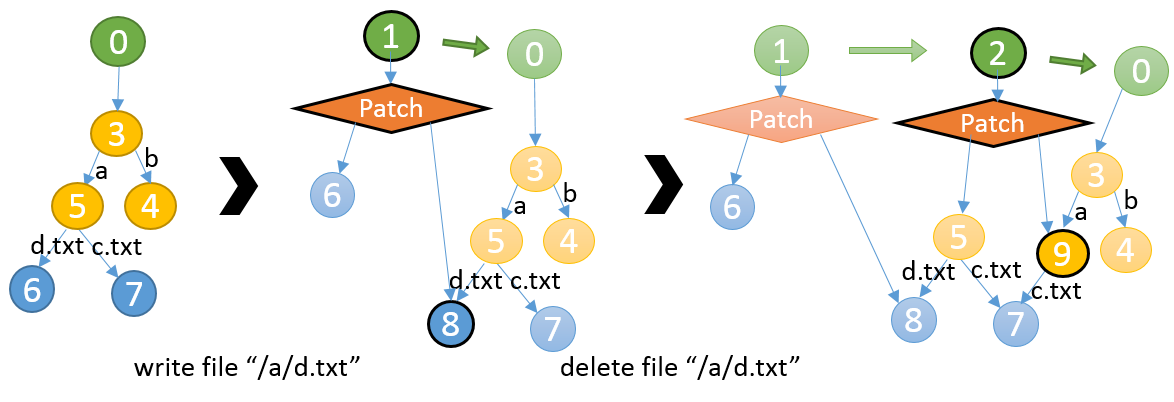
\includegraphics[width=0.8\textwidth]{Chapter-4/figs/fig26.png}
\caption{Using rsync to find unchanged blocks}
\label{fig:rsync}
\end{figure}


	During this process, only the computational overhead is the calculation and matching of rolling checksums. An important property of rolling checksum algorithm is that successive values can be computed in $O(1)$ time, thus ensures all rolling checksums can be calculated using $O(n)$ time. In exchange of this overhead, we may see a significantly decrease in network flow and remote storage when there is duplicate data in buffer.
